% Options for packages loaded elsewhere
\PassOptionsToPackage{unicode}{hyperref}
\PassOptionsToPackage{hyphens}{url}
%
\documentclass[
]{article}
\usepackage{amsmath,amssymb}
\usepackage{iftex}
\ifPDFTeX
  \usepackage[T1]{fontenc}
  \usepackage[utf8]{inputenc}
  \usepackage{textcomp} % provide euro and other symbols
\else % if luatex or xetex
  \usepackage{unicode-math} % this also loads fontspec
  \defaultfontfeatures{Scale=MatchLowercase}
  \defaultfontfeatures[\rmfamily]{Ligatures=TeX,Scale=1}
\fi
\usepackage{lmodern}
\ifPDFTeX\else
  % xetex/luatex font selection
\fi
% Use upquote if available, for straight quotes in verbatim environments
\IfFileExists{upquote.sty}{\usepackage{upquote}}{}
\IfFileExists{microtype.sty}{% use microtype if available
  \usepackage[]{microtype}
  \UseMicrotypeSet[protrusion]{basicmath} % disable protrusion for tt fonts
}{}
\makeatletter
\@ifundefined{KOMAClassName}{% if non-KOMA class
  \IfFileExists{parskip.sty}{%
    \usepackage{parskip}
  }{% else
    \setlength{\parindent}{0pt}
    \setlength{\parskip}{6pt plus 2pt minus 1pt}}
}{% if KOMA class
  \KOMAoptions{parskip=half}}
\makeatother
\usepackage{xcolor}
\usepackage[margin=1in]{geometry}
\usepackage{longtable,booktabs,array}
\usepackage{calc} % for calculating minipage widths
% Correct order of tables after \paragraph or \subparagraph
\usepackage{etoolbox}
\makeatletter
\patchcmd\longtable{\par}{\if@noskipsec\mbox{}\fi\par}{}{}
\makeatother
% Allow footnotes in longtable head/foot
\IfFileExists{footnotehyper.sty}{\usepackage{footnotehyper}}{\usepackage{footnote}}
\makesavenoteenv{longtable}
\usepackage{graphicx}
\makeatletter
\def\maxwidth{\ifdim\Gin@nat@width>\linewidth\linewidth\else\Gin@nat@width\fi}
\def\maxheight{\ifdim\Gin@nat@height>\textheight\textheight\else\Gin@nat@height\fi}
\makeatother
% Scale images if necessary, so that they will not overflow the page
% margins by default, and it is still possible to overwrite the defaults
% using explicit options in \includegraphics[width, height, ...]{}
\setkeys{Gin}{width=\maxwidth,height=\maxheight,keepaspectratio}
% Set default figure placement to htbp
\makeatletter
\def\fps@figure{htbp}
\makeatother
\setlength{\emergencystretch}{3em} % prevent overfull lines
\providecommand{\tightlist}{%
  \setlength{\itemsep}{0pt}\setlength{\parskip}{0pt}}
\setcounter{secnumdepth}{-\maxdimen} % remove section numbering
\newlength{\cslhangindent}
\setlength{\cslhangindent}{1.5em}
\newlength{\csllabelwidth}
\setlength{\csllabelwidth}{3em}
\newlength{\cslentryspacingunit} % times entry-spacing
\setlength{\cslentryspacingunit}{\parskip}
\newenvironment{CSLReferences}[2] % #1 hanging-ident, #2 entry spacing
 {% don't indent paragraphs
  \setlength{\parindent}{0pt}
  % turn on hanging indent if param 1 is 1
  \ifodd #1
  \let\oldpar\par
  \def\par{\hangindent=\cslhangindent\oldpar}
  \fi
  % set entry spacing
  \setlength{\parskip}{#2\cslentryspacingunit}
 }%
 {}
\usepackage{calc}
\newcommand{\CSLBlock}[1]{#1\hfill\break}
\newcommand{\CSLLeftMargin}[1]{\parbox[t]{\csllabelwidth}{#1}}
\newcommand{\CSLRightInline}[1]{\parbox[t]{\linewidth - \csllabelwidth}{#1}\break}
\newcommand{\CSLIndent}[1]{\hspace{\cslhangindent}#1}
\usepackage{float}
\floatplacement{figure}{H}
\ifLuaTeX
  \usepackage{selnolig}  % disable illegal ligatures
\fi
\IfFileExists{bookmark.sty}{\usepackage{bookmark}}{\usepackage{hyperref}}
\IfFileExists{xurl.sty}{\usepackage{xurl}}{} % add URL line breaks if available
\urlstyle{same}
\hypersetup{
  pdftitle={Fitting associate learning models to data},
  pdfauthor={Andrés E. Quiñones},
  hidelinks,
  pdfcreator={LaTeX via pandoc}}

\title{Fitting associate learning models to data}
\author{Andrés E. Quiñones}
\date{2023-12-21}

\begin{document}
\maketitle

\hypertarget{the-boussard-et-al-data-set}{%
\subsection{\texorpdfstring{The Boussard \emph{et al} data
set}{The Boussard et al data set}}\label{the-boussard-et-al-data-set}}

In here I present the statistical model used to estimate reinforcement
learning parameters from data from a reversal learning task. In the
experimental set up, individuals from two experimental treatments are
trained to pick one of two stimuli. Where one of those two options
provides reward in the form of food pellets. The experiments is composed
of 11 reversal blocks, each of these blocks is composed of 30 trial. In
other words, every 30 trials the stimulus that provides reward is
switched. Thus, individuals must reverse their estimate of reward in
order to make adaptive decisions and choose the rewarding stimulus. In
figure \ref{fig:plotBoussard}, I show the proportion of correct choices
for both treatment groups along the trials, and reversal blocks.

\begin{figure}

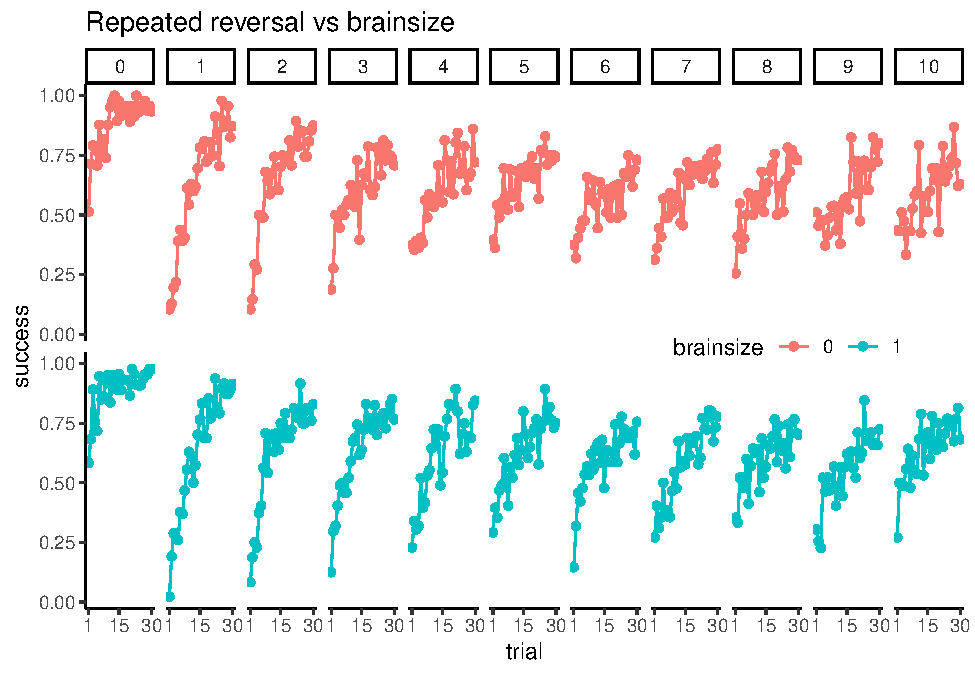
\includegraphics{report_files/figure-latex/plotBoussard-1} \hfill{}

\caption{The Boussard *et al* data-set. Points show the proportion of successes achieved by individuals of both treatment groups along trials and reversal blocks.}\label{fig:plotBoussard}
\end{figure}

In order to evaluate the performance of the model in estimating the
parameter values. I first fit the model parameters to a data-set
obtained by simulation the model with a set of pre-set parameter values.
I then evaluate whether the algorithm correctly estimates these
parameters. The model is based of the Rescorla-Wagner model of
associative learning. Each individual has an estimate of reward for each
stimulus. When two stimuli are presented together, the individual
chooses one of the two with a probability given by the soft-max
distribution. We assume all individuals use the same temperature
parameter \((\tau)\). This parameter is estimated. Once the individual
chooses one of the two stimuli, it updates its estimates of reward
associated with the chosen stimulus. The update is performed every trial
and is given by the product of the \emph{prediction error} \((\delta)\)
and the \emph{speed of learning} \((\alpha)\). The \emph{prediction
error} is calculated as the difference between the reward triggered by
choosing a particular stimulus and the estimation of that reward prior
to the choice. We assume each individual expresses a different
\emph{speed of learning}, and it's given by fixed and random effects.
The treatment group of each individual is the fixed effect. Thus, we
estimate a contribution of the treatment group to the \emph{speed of
learning} of each individual. As for the random effect, we assume the
individual specific contributions to the speed of learning are
distributed as a random variable with a normal distribution. We estimate
the mean and standard deviation of the distribution. The model uses thus
a hierarchical bayesian approach to estimating the parameters of the
Rescorla-Wagner model.

\hypertarget{the-simple-fake-data-set}{%
\subsection{The simple fake data set}\label{the-simple-fake-data-set}}

We first use the model to estimate a simple associative learning task
without any reward reversal. In table \ref{tab:param_simple}, I show the
values of the model parameters to simulate the first data-set. In figure
\ref{fig:simple_dataset}, I show the average frequency of success for
the two treatment groups. In figure \ref{fig:est_simple}, I show the
confidence interval of the parameters estimated, as well as the values
used for the simulations. In fig \ref{fig:ppcheck_simple}, I show how
the data predicted by the estimated parameters compares with the data
simulated from the `real' parameters.

\begin{longtable}[]{@{}lr@{}}
\caption{\label{tab:param_simple} Parameters of the simulated
data-set.}\tabularnewline
\toprule\noalign{}
parameters & values \\
\midrule\noalign{}
\endfirsthead
\toprule\noalign{}
parameters & values \\
\midrule\noalign{}
\endhead
\bottomrule\noalign{}
\endlastfoot
Temperature & 1.0 \\
Mean speed of learning & 0.2 \\
Effect of treatment 0 & -5.0 \\
Effect of treatment 1 & 5.0 \\
St.~dev. of speed of learning & 2.0 \\
\end{longtable}

\begin{figure}

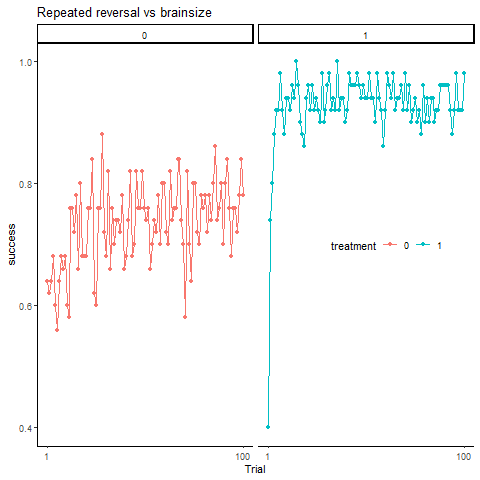
\includegraphics[width=6.67in,]{images/simple_DS} \hfill{}

\caption{Simulated data from a simple associative learning model with two treatment effects. Points represent the frequency of successes among 50 individuals.}\label{fig:simple_dataset}
\end{figure}

\begin{figure}

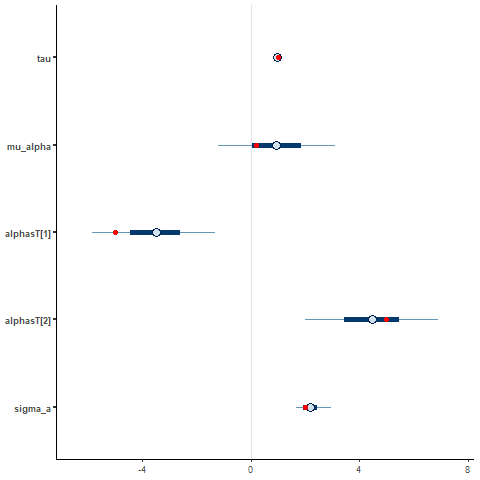
\includegraphics[width=6.67in,]{images/simple_mcmc_intervals} \hfill{}

\caption{ Estimation of the paramerters used to generate the simulated data. Blue bars and lines correspond to the 50 and 90\% credible intervals, respectively. Red points correspond to the real values of the parameteres used in the simulation.}\label{fig:est_simple}
\end{figure}

\begin{figure}

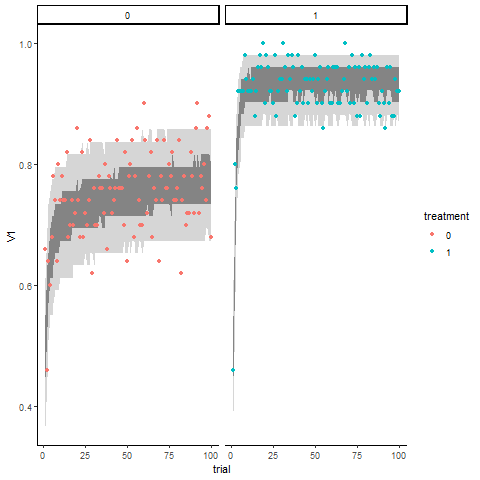
\includegraphics[width=6.67in,]{images/simple_ppchecks} \hfill{}

\caption{Out of sample posterior predictive checks of the bayesian estimation. Points correspond to a simulated data-set using the parameter values shown earlier. Light and dark grey bands correspond to the 50 and 90\% credible interval of predictions made from the posterior distributions.}\label{fig:ppcheck_simple}
\end{figure}

\hypertarget{the-reversal-fake-data-set}{%
\subsection{The reversal fake data
set}\label{the-reversal-fake-data-set}}

Now I presented a date-set simulatd from the model, but including
reversal learning structured in the same way as the Boussard \emph{et
al} experiments. Table \ref{tab:param_rev} shows the parameter values
used for the simulations, fig.~\ref{fig:rev_sim_data} shows the data
simulated from the model, fig.~\ref{fig:rev_sim_interv} shows the
estimation of the parameters together with the'real' value. Finally,
fig.~\ref{fig:ppcheck_rev} shows the predictions from the estimated
parameters together with data simulated with the `real' values.

\begin{longtable}[]{@{}lr@{}}
\caption{\label{tab:param_rev} Parameters of the simulated reversal
learning data-set}\tabularnewline
\toprule\noalign{}
parameters & values \\
\midrule\noalign{}
\endfirsthead
\toprule\noalign{}
parameters & values \\
\midrule\noalign{}
\endhead
\bottomrule\noalign{}
\endlastfoot
Temperature & 1.0 \\
Mean speed of learning & 0.2 \\
Effect of treatment 0 & -2.0 \\
Effect of treatment 1 & 2.0 \\
St.~dev. of speed of learning & 0.5 \\
\end{longtable}

\begin{figure}

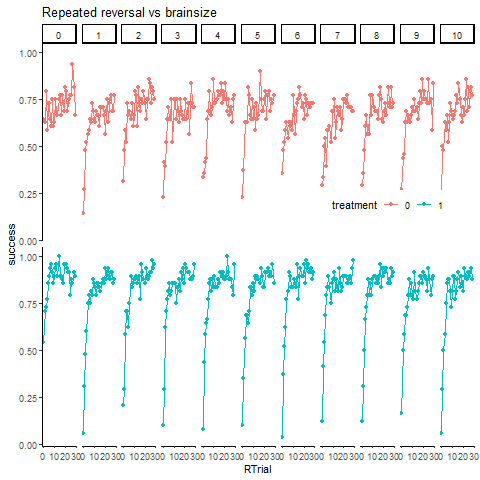
\includegraphics[width=6.67in,]{images/reversal_data} \hfill{}

\caption{Simulated data of the reversal learning model.}\label{fig:rev_sim_data}
\end{figure}

\begin{figure}

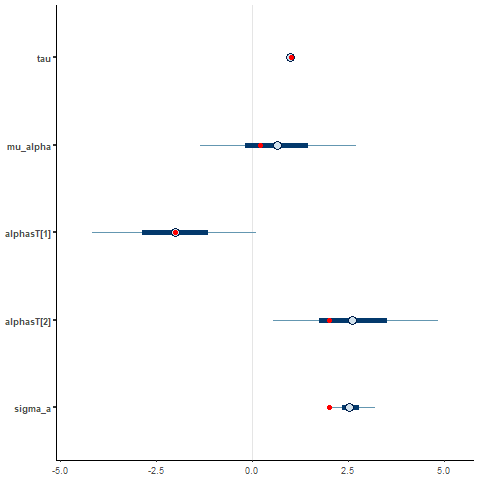
\includegraphics[width=6.67in,]{images/reversal_mcmc_interv} \hfill{}

\caption{Estimated credible intervals and real values of the parameters of the reversal learning model. Blue bars and lines correspond to the 50 and 90\% credible intervals, respectively. Red points correspond to the real values of the parameteres used in the simulation of reversal learning. }\label{fig:rev_sim_interv}
\end{figure}

\begin{figure}

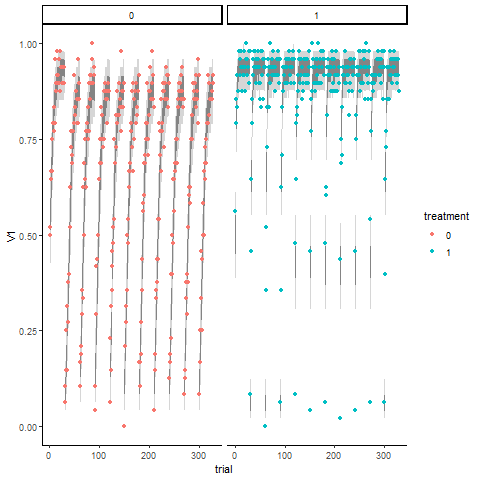
\includegraphics[width=6.67in,]{images/reversal_ppchecks} \hfill{}

\caption{Out of sample posterior predictive checks of the bayesian estimation. Points correspond to a simulated data-set using the parameter values shown earlier from the simulation of reversal learning. Light and dark grey bands correspond to the 50 and 90\% credible interval}\label{fig:ppcheck_rev}
\end{figure}

\hypertarget{fitting-the-model-to-the-boussard-et-al-data-set}{%
\subsection{\texorpdfstring{Fitting the model to the Boussard \emph{et
al} data
set}{Fitting the model to the Boussard et al data set}}\label{fitting-the-model-to-the-boussard-et-al-data-set}}

Now we use the model to fit the parameters to the Boussard \emph{et al}
data-set. Figure \ref{fig:boussard_interv} shows the parameters
estimated and figure \ref{fig:ppchecks_boussard} shows how well the data
fits the predictions from the model. Clearly a model with constant speed
of learning throughout the reversal blocks does not capture well the
desicion-making dynamics.

\begin{figure}

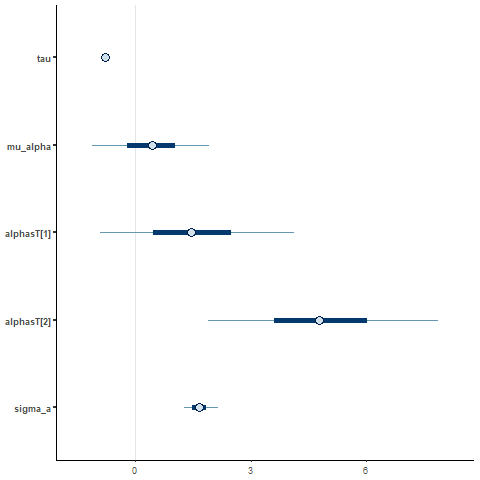
\includegraphics[width=6.67in,]{images/boussard_mcmc_interv} \hfill{}

\caption{Bayesian estimation of parameters to the Boussard *et al* 2020 data-set. Light and dark grey bands correspond to the 50 and 90\% credible interval}\label{fig:boussard_interv}
\end{figure}

\begin{figure}

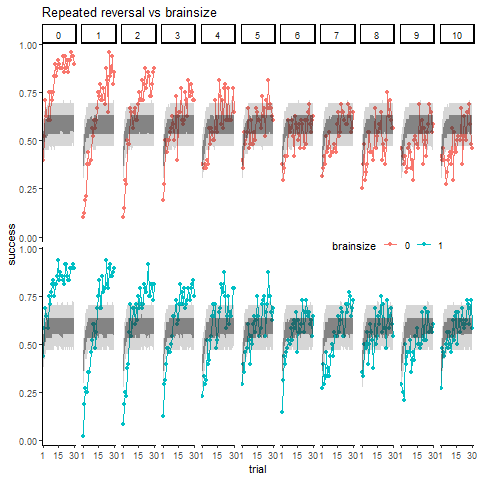
\includegraphics[width=6.67in,]{images/boussard_ppchecks} \hfill{}

\caption{Posterior predictive checks of the bayesian estimation. Points correspond to Boussard *et al* 2020 data-set . Light and dark grey bands correspond to the 50 and 90\% credible interval predicted by the model}\label{fig:ppchecks_boussard}
\end{figure}

\hypertarget{let-fit-a-model-with-different-learning-rates-in-reversal-blocks-to-the-boussard--boussard_brain_2020-data-set}{%
\subsection{Let' fit a model with different learning rates in reversal
blocks to the Boussard (2020) data
set}\label{let-fit-a-model-with-different-learning-rates-in-reversal-blocks-to-the-boussard--boussard_brain_2020-data-set}}

Now we use a model where we allow individuals to have a different
\emph{speed of learning} on each reversal block. To do that, we estimate
a fixed effect of the reversal block on the parameter \(\alpha\). Figure
\ref{fig:interv_rev} shows the estimated parameters including the effect
of reversal block on the \emph{speed of learning}, figure
\ref{fig:ppchecks_boussard_rev} shows how well the model predicts the
data. For some reason, the model estimates a very low \emph{speed of
learning} in the early blocks of reversal. This causes the model to
perform rather poorly in explaining the desicion-making dynamics.

\begin{figure}

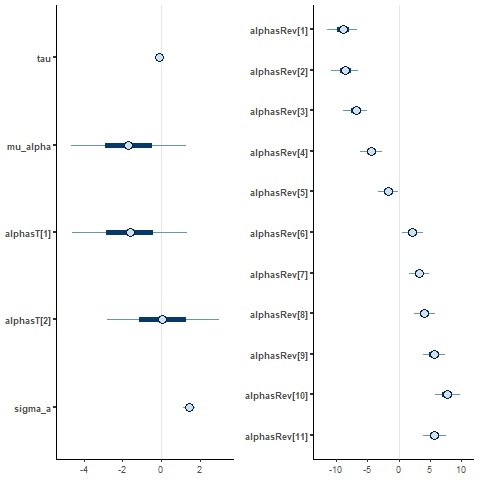
\includegraphics[width=6.67in,]{images/boussard_mcmc_interv_rev} \hfill{}

\caption{Estimated credible intervals of the parameters of the reversal learning model. Blue bars and lines correspond to the 50 and 90\% credible intervals, respectively. Red points correspond to the real values of the parameteres used in the simulation of reversal learning. Panel on the right shows the estimated effect of the reversal blocks on the speed of learning.}\label{fig:interv_rev}
\end{figure}

\begin{figure}

\includegraphics[width=6.67in,]{images/boussardREV_ppchecks} \hfill{}

\caption{Posterior predictive checks of the bayesian estimation for a model with different *speed of learning* on the reversal blocks. Points correspond to Boussard  data-set. Light and dark grey bands correspond to the 50 and 90\% credible interval predicted by the model}\label{fig:ppchecks_boussard_rev}
\end{figure}

\hypertarget{the-reversal-fake-data-set-with-different-learning-rates-in-the-different-reversal-blocks}{%
\subsection{The reversal fake data set with different learning rates in
the different reversal
blocks}\label{the-reversal-fake-data-set-with-different-learning-rates-in-the-different-reversal-blocks}}

\begin{longtable}[]{@{}lr@{}}
\caption{\label{tab:param_rev_meta} Parameters of the simulated reversal
learning data-set}\tabularnewline
\toprule\noalign{}
parameters & values \\
\midrule\noalign{}
\endfirsthead
\toprule\noalign{}
parameters & values \\
\midrule\noalign{}
\endhead
\bottomrule\noalign{}
\endlastfoot
Temperature & 1.0 \\
Mean speed of learning & 0.0 \\
Effect of treatment 0 & -2.0 \\
Effect of treatment 1 & 0.5 \\
St.~dev. of speed of learning & 2.0 \\
Effect of reversal block 1 & 2.0 \\
Effect of reversal block 2 & 1.6 \\
Effect of reversal block 3 & 1.2 \\
Effect of reversal block 4 & 0.8 \\
Effect of reversal block 5 & 0.4 \\
Effect of reversal block 6 & 0.0 \\
Effect of reversal block 7 & -0.4 \\
Effect of reversal block 8 & -0.8 \\
Effect of reversal block 9 & -1.2 \\
Effect of reversal block 10 & -1.6 \\
Effect of reversal block 11 & -2.0 \\
\end{longtable}

\begin{figure}

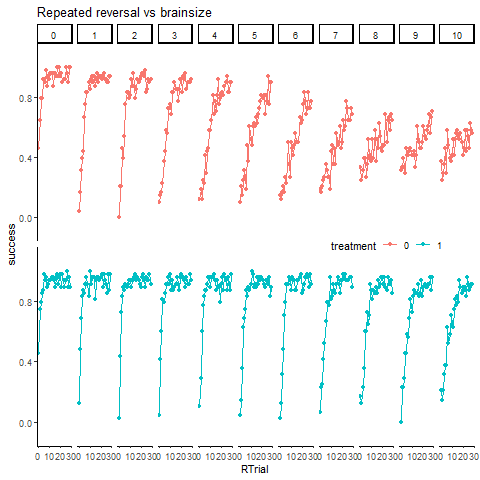
\includegraphics[width=6.67in,]{images/reversal_data_sim_block} \hfill{}

\caption{Simulated data of the reversal learning model.}\label{fig:rev_sim_data_block}
\end{figure}

\begin{figure}

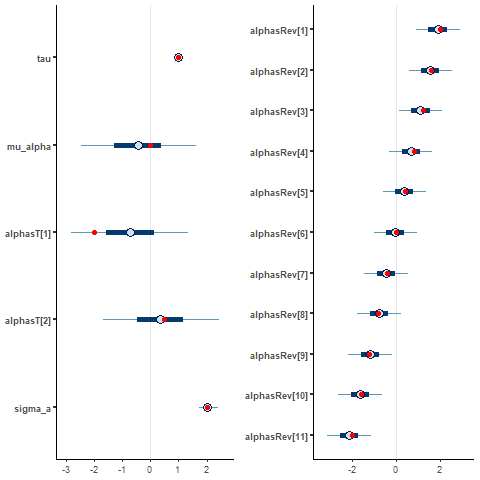
\includegraphics[width=6.67in,]{images/sim_mcmc_interv_rev} \hfill{}

\caption{Estimated credible intervals and real values of the parameters of the reversal learning model. Blue bars and lines correspond to the 50 and 90\% credible intervals, respectively. Red points correspond to the real values of the parameteres used in the simulation of reversal learning. }\label{fig:rev_sim_interv_block}
\end{figure}

\begin{figure}

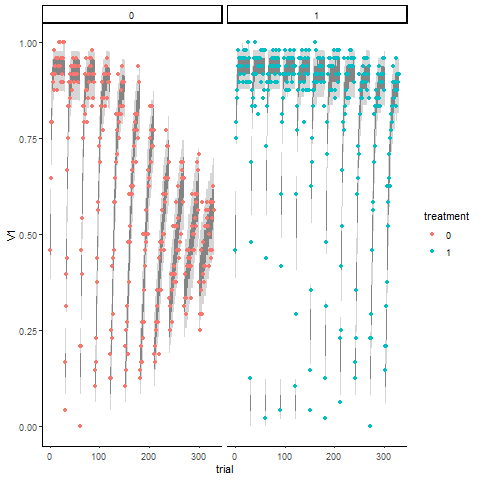
\includegraphics[width=6.67in,]{images/sim_reversal_ppchecks} \hfill{}

\caption{Out of sample posterior predictive checks of the bayesian estimation. Points correspond to a simulated data-set using the parameter values shown earlier from the simulation of reversal learning. Light and dark grey bands correspond to the 50 and 90\% credible interval}\label{fig:ppcheck_rev_sim}
\end{figure}

\hypertarget{fitting-the-model-with-2-treatment-effects}{%
\subsection{Fitting the model with 2 treatment
effects}\label{fitting-the-model-with-2-treatment-effects}}

\hypertarget{boussard--boussard_link_2021-brain-size-v.s.-age}{%
\section{\texorpdfstring{Boussard (2021) brain size \emph{v.s.}
age}{Boussard (2021) brain size v.s. age}}\label{boussard--boussard_link_2021-brain-size-v.s.-age}}

As another example I show now results from fitting the model to the
Boussard (2021) data-set. Where fish from the to brain size experimental
groups are assessed on the effect of age in a single reversal learning
task.

\begin{figure}

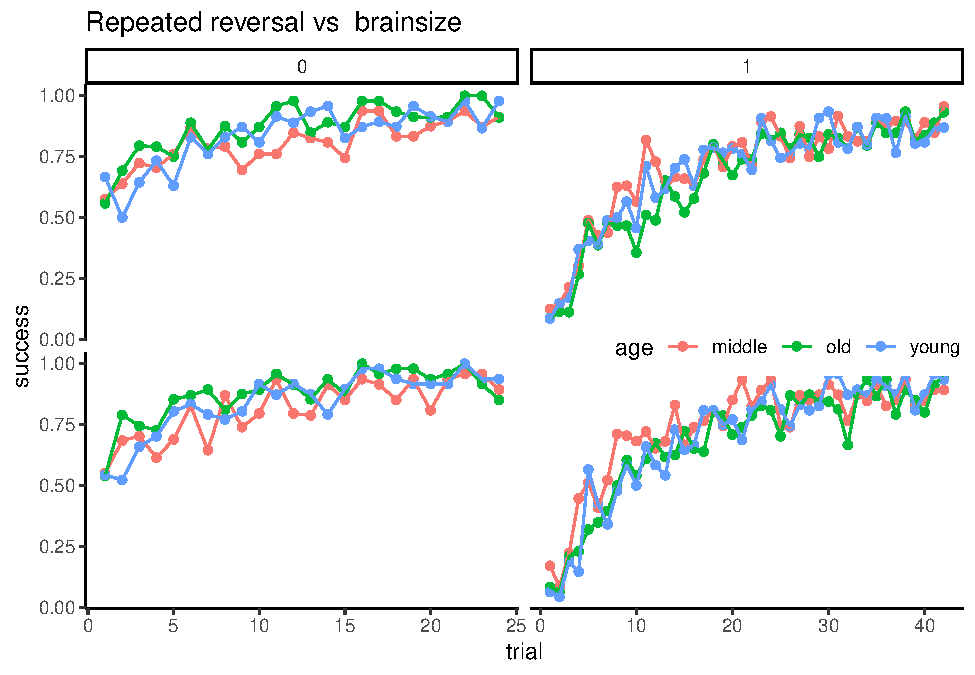
\includegraphics{report_files/figure-latex/unnamed-chunk-7-1} \hfill{}

\caption{Performance of fish according to the two experimental groups  - brain size and age - along the initial and reversal learning}\label{fig:unnamed-chunk-7}
\end{figure}

\begin{figure}

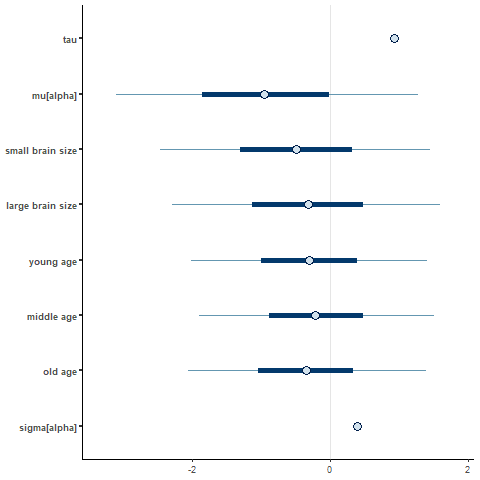
\includegraphics[width=6.67in,]{images/boussard2intervals} \hfill{}

\caption{Bayesian estimation of parameters to the Boussard *et al* 2021 data set. Light and dark grey bands correspond to the 50 and 90\% credible interval}\label{fig:unnamed-chunk-8}
\end{figure}

\begin{figure}

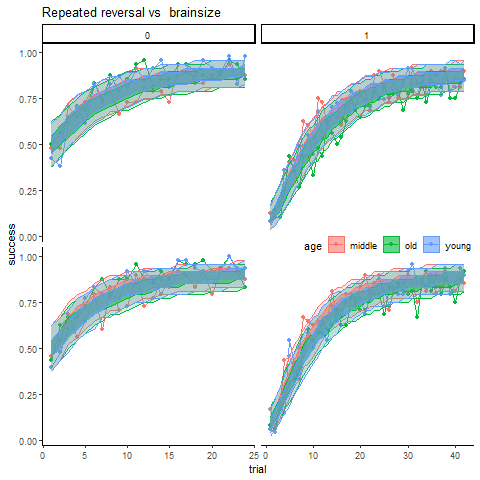
\includegraphics[width=6.67in,]{images/boussard2_ppchecks} \hfill{}

\caption{Posterior predictive checks of the bayesian estimation. Points correspond to Boussard data-set. Light and dark coloured bands correspond to the 50 and 90\% credible interval predicted by the model}\label{fig:unnamed-chunk-9}
\end{figure}

\hypertarget{fitting-the-model-with-2-treatment-effects-and-a-colour-effect}{%
\subsection{Fitting the model with 2 treatment effects and a colour
effect}\label{fitting-the-model-with-2-treatment-effects-and-a-colour-effect}}

\hypertarget{boussard--boussard_link_2021-brain-size-v.s.-age-v.s.-colour}{%
\section{\texorpdfstring{Boussard (2021) brain size \emph{v.s.} age
\emph{v.s.}
colour}{Boussard (2021) brain size v.s. age v.s. colour}}\label{boussard--boussard_link_2021-brain-size-v.s.-age-v.s.-colour}}

As another example I show now results from fitting the model to the
Boussard (2021) data-set. Where fish from the to brain size experimental
groups are assessed on the effect of age in a single reversal learning
task.

\begin{figure}

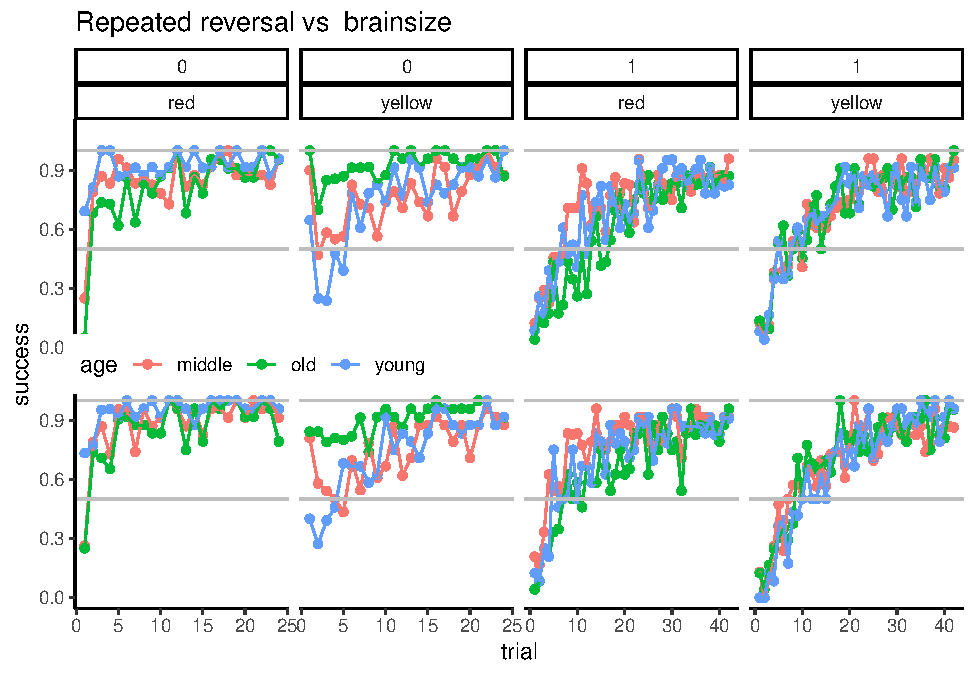
\includegraphics{report_files/figure-latex/unnamed-chunk-10-1} \hfill{}

\caption{Performance of fish according to the two experimental groups  - brain size and age - along the initial and reversal learning}\label{fig:unnamed-chunk-10}
\end{figure}

\begin{figure}

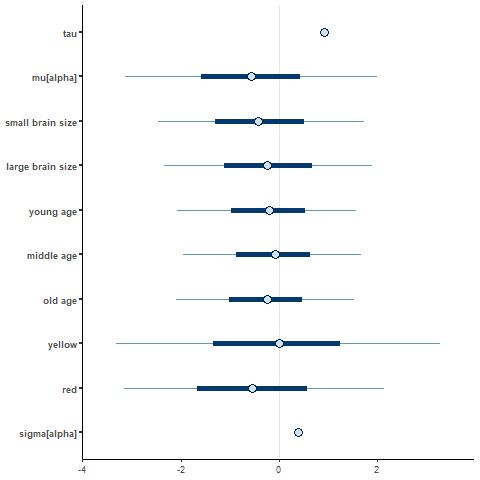
\includegraphics[width=6.67in,]{images/boussard2intervals_col} \hfill{}

\caption{Bayesian estimation of parameters to the Boussard *et al* 2021 data set. Light and dark grey bands correspond to the 50 and 90\% credible interval}\label{fig:unnamed-chunk-11}
\end{figure}

\begin{figure}

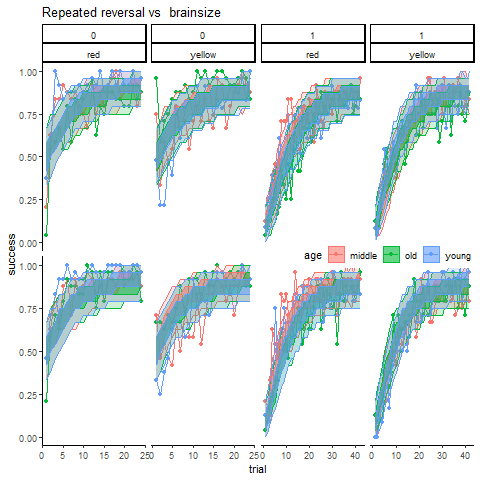
\includegraphics[width=6.67in,]{images/boussard2_ppchecks_colour} \hfill{}

\caption{Posterior predictive checks of the bayesian estimation. Points correspond to Boussard data-set. Light and dark coloured bands correspond to the 50 and 90\% credible interval predicted by the model}\label{fig:unnamed-chunk-12}
\end{figure}

\hypertarget{fitting-the-model-with-2-treatment-effects-influencing-the-temperature-parameter}{%
\subsection{Fitting the model with 2 treatment effects influencing the
temperature
parameter}\label{fitting-the-model-with-2-treatment-effects-influencing-the-temperature-parameter}}

\hypertarget{boussard--boussard_link_2021-brain-size-v.s.-age-1}{%
\section{\texorpdfstring{Boussard (2021) brain size \emph{v.s.}
age}{Boussard (2021) brain size v.s. age}}\label{boussard--boussard_link_2021-brain-size-v.s.-age-1}}

As another example I show now results from fitting the model to the
Boussard (2021) data-set. Where fish from the to brain size experimental
groups are assessed on the effect of age in a single reversal learning
task.

\begin{figure}

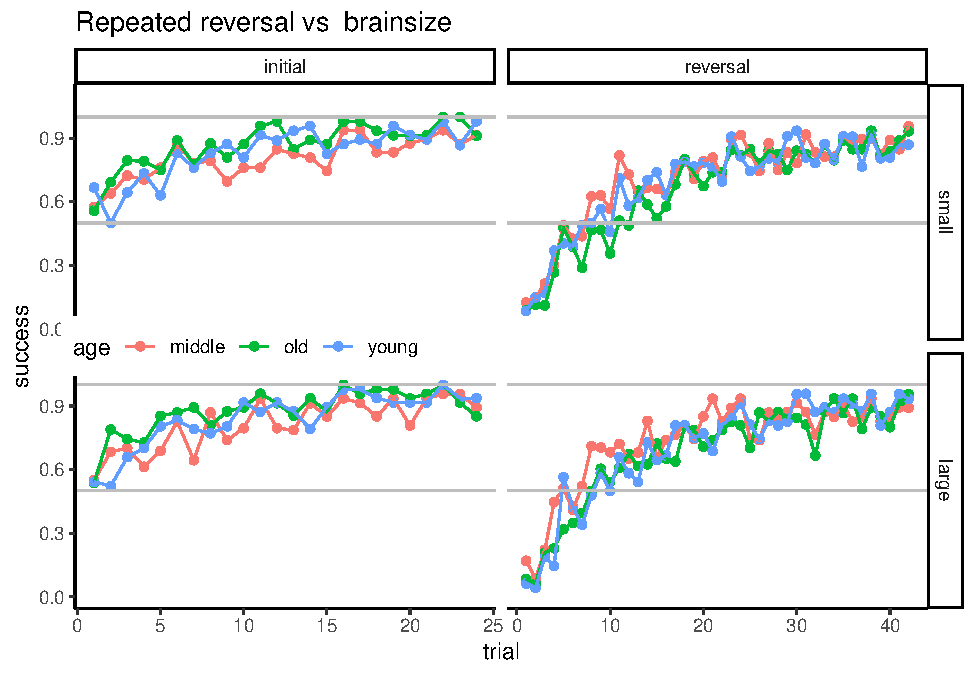
\includegraphics{report_files/figure-latex/unnamed-chunk-13-1} \hfill{}

\caption{Performance of fish according to the two experimental groups  - brain size and age - along the initial and reversal learning}\label{fig:unnamed-chunk-13}
\end{figure}

\begin{figure}

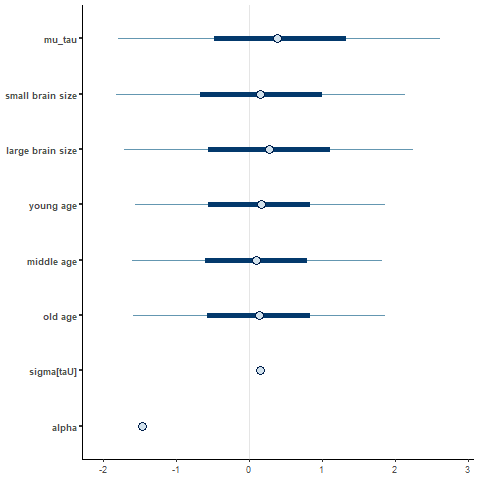
\includegraphics[width=6.67in,]{images/boussard2intervals_tau} \hfill{}

\caption{Bayesian estimation of parameters to the Boussard *et al* 2021 data set. Light and dark grey bands correspond to the 50 and 90\% credible interval}\label{fig:unnamed-chunk-14}
\end{figure}

\begin{figure}

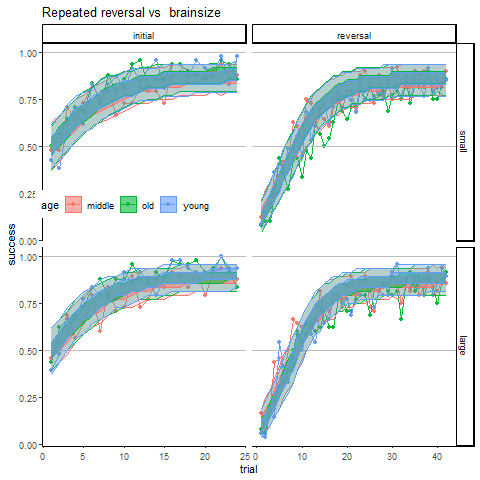
\includegraphics[width=6.67in,]{images/boussard2_ppchecks_tau} \hfill{}

\caption{Posterior predictive checks of the bayesian estimation. Points correspond to Boussard data-set. Light and dark coloured bands correspond to the 50 and 90\% credible interval predicted by the model}\label{fig:unnamed-chunk-15}
\end{figure}

\hypertarget{fitting-the-model-with-2-treatment-effects-influencing-the-temperature-parameter-and-random-effects-on-the-speed-of-learning}{%
\subsection{Fitting the model with 2 treatment effects influencing the
temperature parameter and random effects on the speed of
learning}\label{fitting-the-model-with-2-treatment-effects-influencing-the-temperature-parameter-and-random-effects-on-the-speed-of-learning}}

\hypertarget{boussard--boussard_link_2021-brain-size-v.s.-age-2}{%
\section{\texorpdfstring{Boussard (2021) brain size \emph{v.s.}
age}{Boussard (2021) brain size v.s. age}}\label{boussard--boussard_link_2021-brain-size-v.s.-age-2}}

As another example I show now results from fitting the model to the
Boussard (2021) data-set. Where fish from the to brain size experimental
groups are assessed on the effect of age in a single reversal learning
task.

\begin{figure}

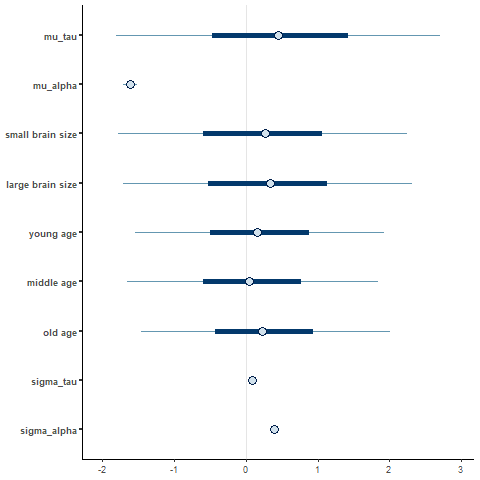
\includegraphics[width=6.67in,]{images/boussard2intervals_tau_alpha} \hfill{}

\caption{Bayesian estimation of parameters to the Boussard *et al* 2021 data set. Light and dark grey bands correspond to the 50 and 90\% credible interval}\label{fig:unnamed-chunk-16}
\end{figure}

\begin{figure}

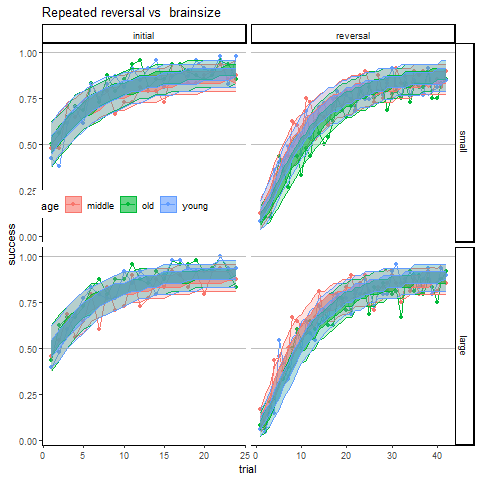
\includegraphics[width=6.67in,]{images/boussard2_ppchecks_tau_alpha} \hfill{}

\caption{Posterior predictive checks of the bayesian estimation. Points correspond to Boussard data-set. Light and dark coloured bands correspond to the 50 and 90\% credible interval predicted by the model}\label{fig:unnamed-chunk-17}
\end{figure}

\hypertarget{fitting-the-model-with-2-treatment-effects-influencing-the-speed-of-learning-and-random-effects-on-the-temperature-parameter}{%
\subsection{Fitting the model with 2 treatment effects influencing the
speed of learning and random effects on the temperature
parameter}\label{fitting-the-model-with-2-treatment-effects-influencing-the-speed-of-learning-and-random-effects-on-the-temperature-parameter}}

\hypertarget{boussard--boussard_link_2021-brain-size-v.s.-age-3}{%
\section{\texorpdfstring{Boussard (2021) brain size \emph{v.s.}
age}{Boussard (2021) brain size v.s. age}}\label{boussard--boussard_link_2021-brain-size-v.s.-age-3}}

As another example I show now results from fitting the model to the
Boussard (2021) data-set. Where fish from the to brain size experimental
groups are assessed on the effect of age in a single reversal learning
task.

\begin{figure}

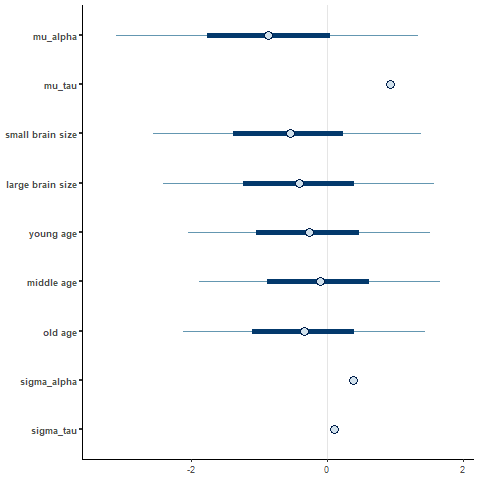
\includegraphics[width=6.67in,]{images/boussard2intervals_alpha_tau} \hfill{}

\caption{Bayesian estimation of parameters to the Boussard *et al* 2021 data set. Light and dark grey bands correspond to the 50 and 90\% credible interval}\label{fig:unnamed-chunk-18}
\end{figure}

\begin{figure}

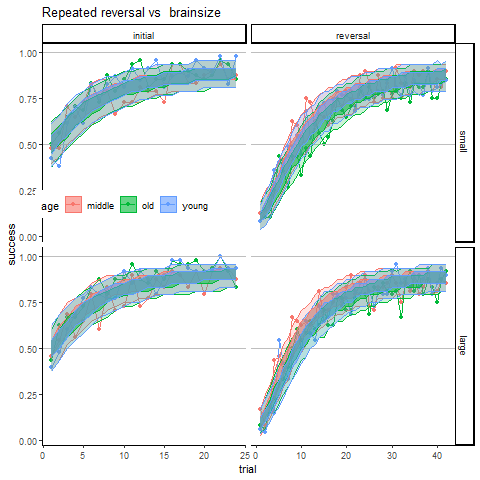
\includegraphics[width=6.67in,]{images/boussard2_ppchecks_alpha_tau} \hfill{}

\caption{Posterior predictive checks of the bayesian estimation. Points correspond to Boussard data-set. Light and dark coloured bands correspond to the 50 and 90\% credible interval predicted by the model}\label{fig:unnamed-chunk-19}
\end{figure}

\hypertarget{references}{%
\subsection*{References}\label{references}}
\addcontentsline{toc}{subsection}{References}

\hypertarget{refs}{}
\begin{CSLReferences}{1}{0}
\leavevmode\vadjust pre{\hypertarget{ref-boussard_Link_2021}{}}%
Boussard, Annika, Mirjam Amcoff, Severine D. Buechel, Alexander
Kotrschal, and Niclas Kolm. 2021. {``The Link Between Relative Brain
Size and Cognitive Ageing in Female Guppies ({Poecilia} Reticulata)
Artificially Selected for Variation in Brain Size.''} \emph{Experimental
Gerontology} 146 (April): 111218.
\url{https://doi.org/10.1016/j.exger.2020.111218}.

\leavevmode\vadjust pre{\hypertarget{ref-boussard_Brain_2020}{}}%
Boussard, Annika, Séverine D. Buechel, Mirjam Amcoff, Alexander
Kotrschal, and Niclas Kolm. 2020. {``Brain Size Does Not Predict
Learning Strategies in a Serial Reversal Learning Test.''} \emph{The
Journal of Experimental Biology} 223 (15): jeb224741.
\url{https://doi.org/10.1242/jeb.224741}.

\end{CSLReferences}

\end{document}
